\section{Zielsetzung}
\label{sec:Ziel}
In diesem Versuch soll das Emissionsspektrum einer Kupfer-Anode untersucht und seine Charakteristika analysiert werden. Des Weiteren wird das Auflösungsvermögen
des Messgeräts und die Absorptionsspektren verschiedener Stoffe betrachtet. 

\section{Theorie}
\label{sec:Theorie}
Röntgenstrahlen können mithilfe einer Elektronenkanone erzeugt werden. Dabei treffen beschleunigte Elektronen auf das Anodenmaterial und geben (kinetische)
Energie an dieses ab. Es wird zwischen zwei Arten der Energieabgabe unterschieden.

\subsection{Kontinuierliches Bremsspektrum}
\label{subsec:Bremsspektrum}
Ein Elektron kann im Coulombfeld eines Atomkerns abgebremst werden,
wodurch es Energie verliert. Diese Energie wird in Form eines Photons (Röntgenquants) emittiert. Da auf diese Weise ein beliebiger Teil der Energie des
Elektrons abgegeben werden kann, entsteht ein kontinuierliches Spektrum, welches \textit{Bremsspektrum} genannt wird.
Bei vollständiger Abgabe der kinetischen Energie $E_\text{kin} = U_\text{B} \cdot e$ des Elektrons wird eine minimale Wellenlänge
\begin{equation}
    \label{eqn:lambda_min}
    \lambda_\text{min} = \frac{h c}{e \cdot U_\text{B}}
\end{equation}
erreicht. Dabei ist $U_\text{B}$ die Beschleunigungsspannung der Apparatur und $e$ die Elementarladung. 
Allgemein gilt der Zusammenhang 
\begin{equation}
    \label{eqn:E_lambda}
    E_\text{Photon} = \frac{h \cdot c}{\lambda}
\end{equation}
zwischen Wellenlänge $\lambda$ und der Energie eines Photons.

\subsection{Charakteristische Röntgenstrahlung} 
\label{subsec:Charakteristische}
Bei der zweiten Form der Energieabgabe wird ein Atom des Anodenmaterials ionisiert, sodass eine Leerstelle in einer inneren Schale des Atoms entsteht. 
Beim Zurückfallen eines Elektrons einer äußeren Schale wird dann wieder ein Phtoton emittiert. Das Elektron kann jedoch nur diskrete Energien abgeben,
welche der Differenz zwischen den Energieniveaus der Elektronen der verschiedenen Schalen entspricht, wodurch die \textit{charakteristische Röntgenstrahlung}
entsteht. Die durch diesen Effekt verursachten Peaks im Röntgenspektrum eines Materials werden mit $K_\alpha$, $K_\beta$, $L_\alpha$ usw. bezeichnet.
Der Index des Bezeichners gibt an, von welcher Position das Elektron auf die $K$-, $L$-, $M$- ... Schale absinkt.

Die Frequenz des emittierten Photons lässt sich mittels der Energiedifferenz der Schalen $m$ und $n$ zu $h \nu = E_m - E_n$ bestimmen. 
Die Bindungsenergie eines Elektrons auf der $n$-ten Schale ergibt sich zu 
\begin{equation}
    \label{eqn:Bindungsenergie}
    E_n = -R_\infty z^2_\text{eff} \cdot \frac{1}{n^2}.
\end{equation}
Die effektive Kernladungszahl $z_\text{eff} = z - \sigma$ beschreibt die Abschirmung der realen Kernladungszahl $z$ durch andere Elektronen mit der 
Abschirmungskonstanten $\sigma$, welche für jedes Elektron des Atoms empirisch bestimmt werden kann. Die \textit{Rydbergenergie} beträgt 
$R_\infty = \qty{13.6}{\electronvolt}$.  

Aufgrund dessen, dass die Abschirmungskonstante für verschiedene Elektronen gleicher Schale abweichen kann, gibt es zu den Übergängen zwischen zwei Schalen
mehrere mögliche Energiedifferenzen, weshalb sich die Peaks eines solchen Übergangs in eine Feinstruktur von mehreren eng beieinander liegenden Peaks
aufspalten lässt, die in diesem Versuch jedoch nicht aufgelöst werden kann.

\subsection{Absorptionsspektren}
\label{subsec:Absorption}
Treffen Röntgenstrahlen (Photonen) auf Materie, so können diese absorbiert werden.
In diesem Versuch haben die Elektronen eine kinetische Energie von $E_\text{kin} = \qty{35}{\kilo\electronvolt}$, die sie maximal übertragen können. 
Bei Röntgenstrahlen mit einer Energie unter $\qty{1}{\mega\electronvolt}$ sind der Compton- und Photoeffekt die maßgeblichen Prozesse der Absorption.
Bei zunehmender Energie nimmt der Absorptionskoeffizient (Maß für die Stärke der Absorption) ab. Übersteigt jedoch die Photonenenergie die Bindungsenergie
eines Elektrons einer Schale, steigt der Absorptionskoeffizient sprunghaft. Es entsteht eine \glqq Kante\grqq{}, dessen Lage mit der Bindungsenergie des
Elektrons übereinstimmt. Diese \textit{Absorptionsenergien} werden nach der Schale, aus welcher das Elektron stammt bezeichnet. Auch hier gibt es eine
Feinstruktur, die in \autoref{fig:Absorption} zu sehen ist.

\begin{figure}
    \centering
    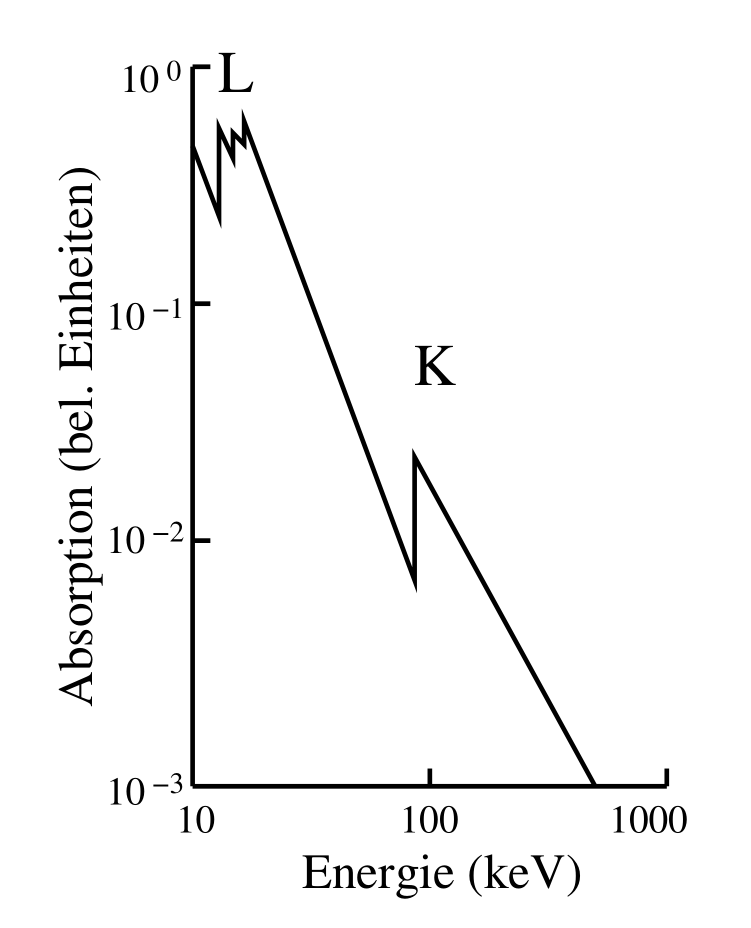
\includegraphics[width = 0.3\textwidth]{content/Absorption.png}
    \caption{Schematische Darstellung der Absorption von Röntgenstrahlen. \cite{v602}}
    \label{fig:Absorption}
\end{figure}

\subsection{Bestimmung der Abschirmkonstanten}
\label{subsec:Abschirmkonstante}
Für Kupfer lassem sich die Abschirmkonstanten $\sigma_1$, $\sigma_2$ und $\sigma_3$ aus den Emissionsenergien der $K_\alpha$- und $K_\beta$-Linie bestimmen.
Eine Abschätzung ergibt die Zusammenhänge 
\begin{align}
    \label{eqn:Sigma_Kupfer}
    E_{K \text{, abs}} &= R_\infty (z - \sigma_1)^2 \\
    \label{eqn:Sigma_Kupfer2}
    E_{K \text{,} \alpha} &= R_\infty \frac{1}{n^2} (z - \sigma_1)^2 - R_\infty \frac{1}{m^2} (z - \sigma_2)^2 \\
    \label{eqn:Sigma_Kupfer3}
    E_{K \text{,} \beta} &= R_\infty \frac{1}{n^2} (z - \sigma_1)^2 - R_\infty \frac{1}{l^2} (z - \sigma_3)^2, 
\end{align}
aus denen sich mit $n = 1$, $m = 2$ und $l = 3$ und dem Wert der Absorptionsenergie $E_{K\text{, abs}}$ die Abschirmkonstanten bestimmen lassen.

Auch bei der Betrachtung des Absorptionsspektrums eines Stoffes lassen sich Abschirmkonstanten bestimmen. 
Für Elektronen der $K$-Schale lässt sich aus der Lage der $K$-Kante des Absorptionsspektrums die Abschirmkonstante $\sigma_{K, \text{abs}}$ zu 
\begin{equation}
    \label{eqn:Sigma_K}
    \sigma_K = z - \sqrt{\frac{E_K}{R_\infty} - \frac{\alpha^2 z^4}{4}}
\end{equation}
bestimmen, wobei $\alpha$ die Sommerfeldsche Feinstrukturkonstante ist.

\subsection{Untersuchung der Spektren mithilfe der Braggreflexion}
\label{subsec:Bragg}
Mithilfe der Braggreflexion lässt sich die Energie und somit auch die Wellenlänge $\lambda$ der untersuchten Röntgenstrahlung bestimmen. 
Das einfallende Röntgenlicht wird dabei an unterschiedlichen Ebenen eines Kristalls reflektiert, was zu Gangunterschieden führt. Durch einfache
geometrische Überlegungen lässt sich die Braggbedingung
\begin{equation}
    \label{eqn:Bragg}
    2 \, d \cdot \symup{sin} \, \theta = n \, \lambda \qquad , n \in \mathbb{N}
\end{equation}
feststellen, die den Fall der konstruktiven Interferenz einer Wellenlänge $\lambda$ unter einem Einstrahlungswinkel $\theta$ beschreibt.
Die Gitterkonstante ist im Falle des verwendeten LiF-Kristalls $d = \qty{201.4}{\pico\metre}$.
